\documentclass[12pt]{article} 
\usepackage[utf8]{inputenc}
\usepackage{geometry}
\geometry{letterpaper}
\usepackage{graphicx} 
\usepackage{parskip}
\usepackage{booktabs}
\usepackage{array} 
\usepackage{paralist} 
\usepackage{verbatim}
\usepackage{subfig}
\usepackage{fancyhdr}
\usepackage{sectsty}
\usepackage{enumitem}
\usepackage{empheq}

\pagestyle{fancy}
\renewcommand{\headrulewidth}{0pt} 
\lhead{}\chead{}\rhead{}
\lfoot{}\cfoot{\thepage}\rfoot{}


%%% ToC (table of contents) APPEARANCE
\usepackage[nottoc,notlof,notlot]{tocbibind} 
\usepackage[titles,subfigure]{tocloft}
\renewcommand{\cftsecfont}{\rmfamily\mdseries\upshape}
\renewcommand{\cftsecpagefont}{\rmfamily\mdseries\upshape} %

\usepackage{amsmath}
\usepackage{amssymb}
\usepackage{mathtools}
\usepackage{empheq}
\usepackage{xcolor}
\usepackage{bbm}
\usepackage{tikz}
\usepackage{pgfplots}
\pgfplotsset{compat=1.18}

\newcommand{\ans}[1]{\boxed{\text{#1}}}
\newcommand{\vecs}[1]{\langle #1\rangle}
\renewcommand{\hat}[1]{\widehat{#1}}
\newcommand{\F}[1]{\mathcal{F}(#1)}
\renewcommand{\P}{\mathbb{P}}
\newcommand{\R}{\mathbb{R}}
\newcommand{\E}{\mathbb{E}}
\newcommand{\Z}{\mathbb{Z}}
\newcommand{\ind}{\mathbbm{1}}
\newcommand{\qed}{\quad \blacksquare}
\newcommand{\brak}[1]{\left\langle #1 \right\rangle}
\newcommand{\bra}[1]{\left\langle #1 \right\vert}
\newcommand{\ket}[1]{\left\vert #1 \right\rangle}
\newcommand{\mfX}{\mathfrak{X}}

\title{APMA 1690: Quiz 2}
\author{Milan Capoor}
\date{}

\begin{document}
\maketitle
\section*{Problem 1}
    \emph{Consider an irreducible and aperiodic Markov chain $\{X_n\}_{n=0}^\infty$ with state space $\{1, 2, 3, 4\}$ and transition matrix}
    \[P = \begin{pmatrix}
        0 & 1/2 & 0 & 1/2\\
        1/3 & 1/3 & 1/3 & 0\\
        0 & 1/2 & 0 & 1/2\\
        1/2 & 0 & 1/2 & 0
    \end{pmatrix}\]

    \begin{enumerate}[label=(\alph*)]
        \item \emph{(2 points) Write down the system of equations (including inequalities) for the stationary
        distribution $\pi = (\pi_1, \pi_2, \pi_3, \pi_4)$. NO NEED TO SOLVE IT. [Do not write the equations
        in a matrix form. I would like to see each equation explicitly.]}

            \color{blue}
                Since the MC is irreducible and has a finite state space, it has a unique stationary distribution $\pi$ given by
                \[\pi^T = P^T \vec\pi\]
                \[\begin{pmatrix}
                    \pi_1 & 
                    \pi_2 &
                    \pi_3 &
                    \pi_4
                \end{pmatrix} = \begin{pmatrix}
                    \pi_1 & 
                    \pi_2 &
                    \pi_3 &
                    \pi_4
                \end{pmatrix}\begin{pmatrix}
                    0 & 1/2 & 0 & 1/2\\
                    1/3 & 1/3 & 1/3 & 0\\
                    0 & 1/2 & 0 & 1/2\\
                    1/2 & 0 & 1/2 & 0
                \end{pmatrix}\]
                \begin{empheq}[box=\fbox]{align*}
                    \pi_1 &= \frac{1}{3}\pi_2 + \frac{1}{2}\pi_4\\
                    \pi_2 &= \frac{1}{2}\pi_1 + \frac{1}{3}\pi_2 + \frac{1}{2}\pi_3\\
                    \pi_3 &= \frac{1}{3}\pi_2 + \frac{1}{2}\pi_4\\
                    \pi_4 &= \frac{1}{2}\pi_1 + \frac{1}{2}\pi_3
                \end{empheq}
            \color{black}

        \item \emph{(1 point) Determine the limit (express it in terms of $\pi_i$'s)}
        \[\lim_{n\to \infty}\P(X_n = 1)\]

            \color{blue}
                $\{X_n\}_{n=0}^\infty$ is an irreducible, aperiodic, Markov chain with a finite state space. By the Ergodic Theorem, 
                \[\lim_{n \to \infty}\P(X_n = x_j) = \pi(x_j)\]
                so 
                \begin{align*}
                    \lim_{n\to \infty}\P(X_n = 1) &= \pi(1) = \boxed{\frac{1}{3}\pi_2 + \frac{1}{2}\pi_4}\\
                \end{align*}
            \color{black}

        \item \emph{(1 point) Determine the value of $v$ in the following equation (express them in terms of
        $\pi_i$'s)}
        \[\P\left\{\omega \in \Omega: \lim_{n\to \infty} \frac{1}{n}\sum_{i=1}^n \ind_{\{X_i(\omega) = 1 \text{ or } 2\}} = v\\\right\} = 1\]
        \emph{where $(\Omega, \P)$ is the underlying probability space.}

            \color{blue}
                The MC is irreducible and has a finite state space so we can use the 2nd Ergodic Theorem. Let $f: \mfX \to \R$ such that $f(X_i) = \ind_{\{X_i = 1 \text{ or } 2\}}$. Then, 
                \[\sum_{x \in \mfX} \pi(x) \cdot \big\vert f(x)\big\vert = \sum_{x \in \mfX} \pi(x) \cdot \ind_{\{x = 1 \text{ or } 2\}} = \pi(x_1) + \pi(x_2)\]

                Since the MC is also aperiodic, we can use the 1st Ergodic Theorem to get
                \[\pi(x_1) + \pi(x_2) = \lim_{n\to \infty} \P(X_n = x_1) + \P(X_n = x_n) \leq 2 < \infty \]
                so 
                \[\sum_{x \in \mfX} \pi(x) \cdot \big\vert f(x)\big\vert < \infty\]
                so 
                \[\P\left\{\omega \in \Omega: \lim_{n\to \infty} \frac{1}{n}\sum_{i=1}^n \ind_{\{X_i(\omega) = 1 \text{ or } 2\}} = \sum_{x \in \mfX} \pi(x) \ind_{\{x = 1 \text{ or } 2\}}\\\right\} = 1\]

                Thus,
                \[v =  \sum_{x \in \mfX} \pi(x) \ind_{\{x = 1 \text{ or } 2\}} = \boxed{\pi(x_1) + \pi(x_2)}\]
            \color{black}

    \end{enumerate}

\pagebreak

\section*{Problem 2}
    \emph{(2 point) Suppose $\{X_n\}_{n=0}^\infty$ is a homogeneous Markov chain taking values in $\mfX = \{x_1, x_2, \dots,\; x_7\}$, and its transition matrix is the following}
    \[P = \begin{pmatrix}
        0.3 & 0 & 0 & 0 & 0.7 & 0 & 0\\
        0.1 & 0.2 & 0.3 & 0.4 & 0 & 0 & 0\\
        0 & 0 & 0.5 & 0.5 & 0 & 0 & 0\\
        0 & 0 & 0 & 0.5 & 0 & 0.5 & 0\\
        0.6 & 0 & 0 & 0 & 0.4 & 0 & 0\\
        0 & 0 & 0 & 0 & 0 & 0.2 & 0.8\\
        0 & 0 & 0 & 1 & 0 & 0 & 0\\
    \end{pmatrix}\]
    \emph{Is this Markov chain irreducible? Justify your answer.}

    \color{blue}
        The transition matrix can be represented by the (unlabelled but weighted) directed graph:
        \begin{center}
            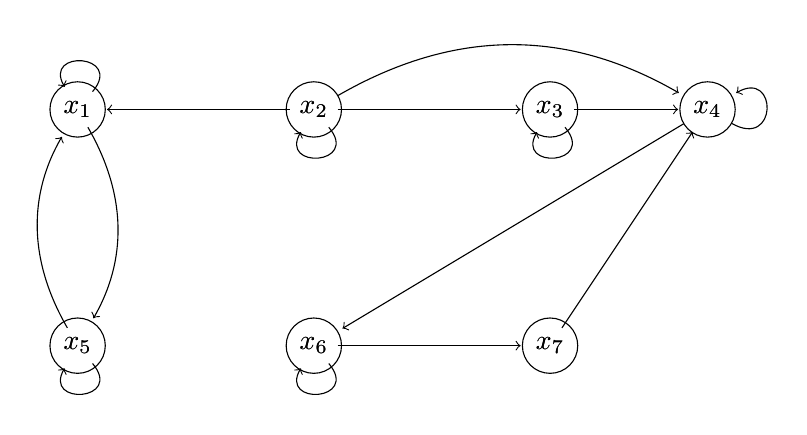
\begin{tikzpicture}
                \node (X1) at (0, 3){$x_1$};
                \node (X2) at (3, 3){$x_2$};
                \node (X3) at (6, 3){$x_3$};
                \node (X4) at (8, 3){$x_4$};
                \node (X5) at (0, 0){$x_5$};
                \node (X6) at (3, 0){$x_6$};
                \node (X7) at (6, 0){$x_7$};
            
                \draw (X1) circle (10pt) node{$x_1$};
                \draw (X2) circle (10pt) node{$x_2$};
                \draw (X3) circle (10pt) node{$x_3$};
                \draw (X4) circle (10pt) node{$x_4$};
                \draw (X5) circle (10pt) node{$x_5$};
                \draw (X6) circle (10pt) node{$x_6$};
                \draw (X7) circle (10pt) node{$x_7$};
            
                \draw[->, shorten >= 2pt] (X1) to [out=50,in=120, looseness=5] (X1);
                \draw[->, shorten >= 2pt] (X2) to [out=-50,in=-120, looseness=5] (X2);
                \draw[->, shorten >= 2pt] (X3) to [out=-50,in=-120, looseness=5] (X3);
                \draw[->, shorten >= 2pt] (X4) to [out=-30,in=30, looseness=5] (X4);
                \draw[->, shorten >= 2pt] (X5) to [out=-50,in=-120, looseness=5] (X5);
                \draw[->, shorten >= 2pt] (X6) to [out=-50,in=-120, looseness=5] (X6);
        
            
                \draw[->, shorten >= 4pt] (X1) to [bend left] (X5);
                \draw[->, shorten >= 4pt] (X5) to [bend left] (X1);
                \draw[->, shorten >= 2pt] (X2) -- (X1);
                \draw[->, shorten >= 2pt] (X2) -- (X3);
                \draw[->, shorten >= 2pt] (X2) to [bend left] (X4);
                \draw[->, shorten >= 2pt] (X3) -- (X4);
                \draw[->, shorten >= 2pt] (X4) -- (X6);
                \draw[->, shorten >= 2pt] (X7) -- (X4);
                \draw[->, shorten >= 2pt] (X6) -- (X7);
            \end{tikzpicture}
        \end{center}

        We proved in HW 6 that a Markov Chain  is irreducible if and only if $\forall x_i, x_j \in \mfX$, there is a directed path from $x_i \to x_j$ and a directed path from $x_j \to x_i$.

        The diagram helps make it clear that this Markov chain is \boxed{\text{not}} irreducible. Notice that there is no directed path from $x_1 \to x_2$ -- just from $x_2 \to x_1$. 

    \color{black}

\pagebreak

\section*{Problem 3}
    \emph{When the irreducibility assumption fails, a homogeneous Markov chain may have infinitely
    many stationary distributions. For example, suppose $\{X_n\}_{n=0}^\infty$ is a homogeneous Markov
    chain taking values in $\mfX = {x_1, x_2, x_3}$, and its transition probability matrix is the following}
    \[P = \begin{pmatrix}
        1/4 & 3/4 & 0\\
        3/4 & 1/4 & 0\\
        0 & 0 & 1
    \end{pmatrix}\]

    \begin{enumerate}[label=(\alph*)]
        \item \emph{(2 points) Prove that the Markov chain $\{X_n\}_{n=0}^\infty$ is reducible (i.e., not irreducible).}
        
            \color{blue}
                This transition matrix can be represented by the graph 
                \begin{center}
                    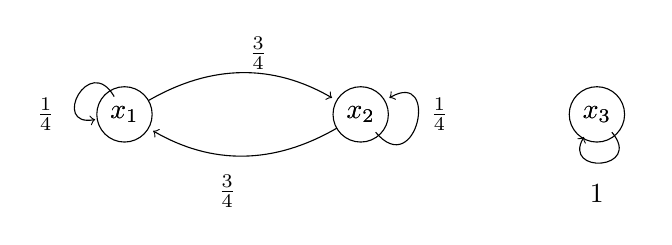
\begin{tikzpicture}
                        \node (X1) at (0, 3){$x_1$};
                        \node (X2) at (3, 3){$x_2$};
                        \node (X3) at (6, 3){$x_3$};

                        \draw (X1) circle (10pt) node{$x_1$};
                        \draw (X2) circle (10pt) node{$x_2$};
                        \draw (X3) circle (10pt) node{$x_3$};

                        \draw[->, shorten >= 2pt] (X1) to [out=120,in=190, looseness=5] (X1) node[xshift=-1cm]{$\frac{1}{4}$};
                        \draw[->, shorten >= 2pt] (X2) to [out=-50,in=30, looseness=5] (X2) node[xshift=1cm]{$\frac{1}{4}$};
                        \draw[->, shorten >= 2pt] (X3) to [out=-50,in=-120, looseness=5] (X3) node[yshift=-1cm]{$1$};

                        \draw[->, shorten >= 2pt] (X2) to [bend left] (X1) node[xshift=1cm, yshift=-0.8cm]{$\frac{3}{4}$};
                        \draw[->, shorten >= 2pt] (X1) to [bend left] (X2) node[xshift=-1cm, yshift=0.6cm]{$\frac{3}{4}$};
                    \end{tikzpicture}
                \end{center}
                
                Clearly, there is no path between $x_1$ and $x_3$ nor between $x_2$ and $x_3$ so the MC is reducible. $\qed$
            \color{black}

        \item \emph{(2 points) Find all the stationary distributions of this Markov chain.}
        
            \color{blue}
                The stationary distributions are given by $\pi^T = \pi^T P$.  
                \begin{gather*}
                    \begin{pmatrix}
                        \pi(x_1) &
                        \pi(x_2) &
                        \pi(x_3)
                    \end{pmatrix} = \begin{pmatrix}
                        \pi(x_1) &
                        \pi(x_2) &
                        \pi(x_3)
                    \end{pmatrix} \begin{pmatrix}
                        1/4 & 3/4 & 0\\
                        3/4 & 1/4 & 0\\
                        0 & 0 & 1
                    \end{pmatrix}\\
                    \begin{cases}
                        \pi(x_1) = \frac{1}{4}\pi(x_1) + \frac{3}{4}\pi(x_2)\\
                        \pi(x_2) = \frac{3}{4}\pi(x_1) + \frac{1}{4}\pi(x_2)\\
                        \pi(x_3) = \pi(x_3)
                    \end{cases} \implies \begin{cases}
                        \pi(x_1) = \pi(x_2)\\
                        \pi(x_3) = \pi(x_3)
                    \end{cases}
                \end{gather*}
                Since the Markov Chain is reducible, there is not a unique stationary distribution.
    
                Adding in the condition that $\pi(x_1) + \pi(x_2) + \pi(x_3) = 1$, we get 
                \[\boxed{\begin{cases}
                    \pi(x_1) = \pi(x_2) = \frac{1-\pi(x_3)}{2}\\
                    \pi(x_3) \; \text{ free}
                \end{cases}}\]
            
            \color{black}

    \end{enumerate} 


\end{document}